\documentclass[main.tex]{subfiles}

\begin{document}

\paragraph{Excersice 1}
Identify from the follwoing graphic the functions that match with the following descriptions:

\begin{minipage}[c]{0.45\textwidth}
    \centering
    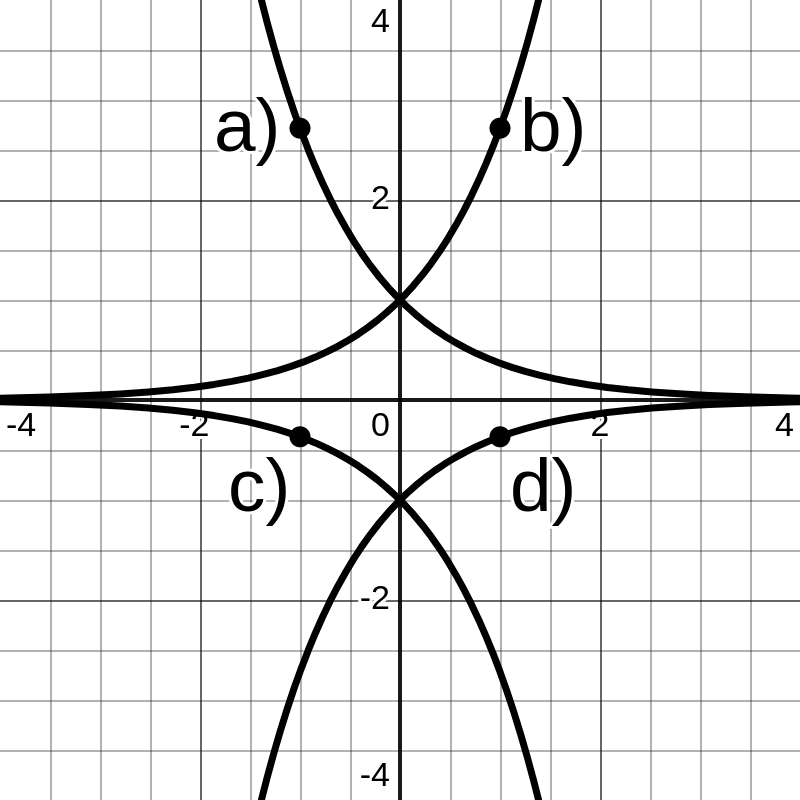
\includegraphics[width=\textwidth]{../imgs/exp-log/exponentials.png}
\end{minipage}
\begin{minipage}[c]{0.45\textwidth}
\begin{itemize}
    \item Exponential growth 
    \item Exponential decay
    \item The function goes to minus infinity when the domain goes to infinity ($f(x)\to-\infty$ when $x\to\infty$)
    \item  The function goes to minus infinity when the domain goes to -infinity ($f(x)\to-\infty$ when $x\to-\infty$)
\end{itemize}
\end{minipage}

\paragraph{Excersice 2}
Use the properties of logarithms to expand the following expression, \[\log\qty[\frac{(x+7)^5}{\sqrt[3]{x^4}}].\]

\paragraph{Exercise 3}
Modify the exponential function ($e^x=\exp[x]$) to move it 3 units to the left and 5 units up.

\paragraph{Exercise 4}
Modify the logarithmic function ($\log_a[x]$) to move it 4 units to the right and 9 untis down.

\paragraph{Exercise 5}
Write the Lograithm law of a quotient.

\paragraph{Exercise 6}
Use the laws of logarithms to expand the following expression, \[\log_e\qty(\frac{(xy)^3}{z^6})=\ln\qty(\frac{(xy)^3}{z^6})\]

\paragraph{Exercise 7}
Determine the horizontal asymptote of the following function, \[f(x)=e^{3x}\qty(\exp\qty[3x]-1)-10\]

\paragraph{Exercise 8}
Find the intersection point between the line $f(x)=e$ and the following function, \[f(x)=\exp\qty[2x]-6\]

\paragraph{Exercise 9}
Solve the equation \[\log\qty(x^2+1)=\log\qty(x-2)+\log(x+3)\]

\end{document}
